\section{Process}

\subsection{Sekvensdiagrammer}
Der er udarbejdet et sekvensdiagram for hver use case. Et sekvensdiagram viser hvordan systemets dele og aktører interagerer med hinanden, og hvilke processer der sker ved disse interaction. Det er beskrevet som sekventiel process og der illustreret diagrammet også hvilke rækkefølge processerne skal eksekveres i. 
Fordi at simplificeret store sekvensdiagrammer gør nogle af dem brug af andre use case, dette ses fx. i sekvensdiagrammet for use case 1. 

\subsection{Konditionering - UC1}
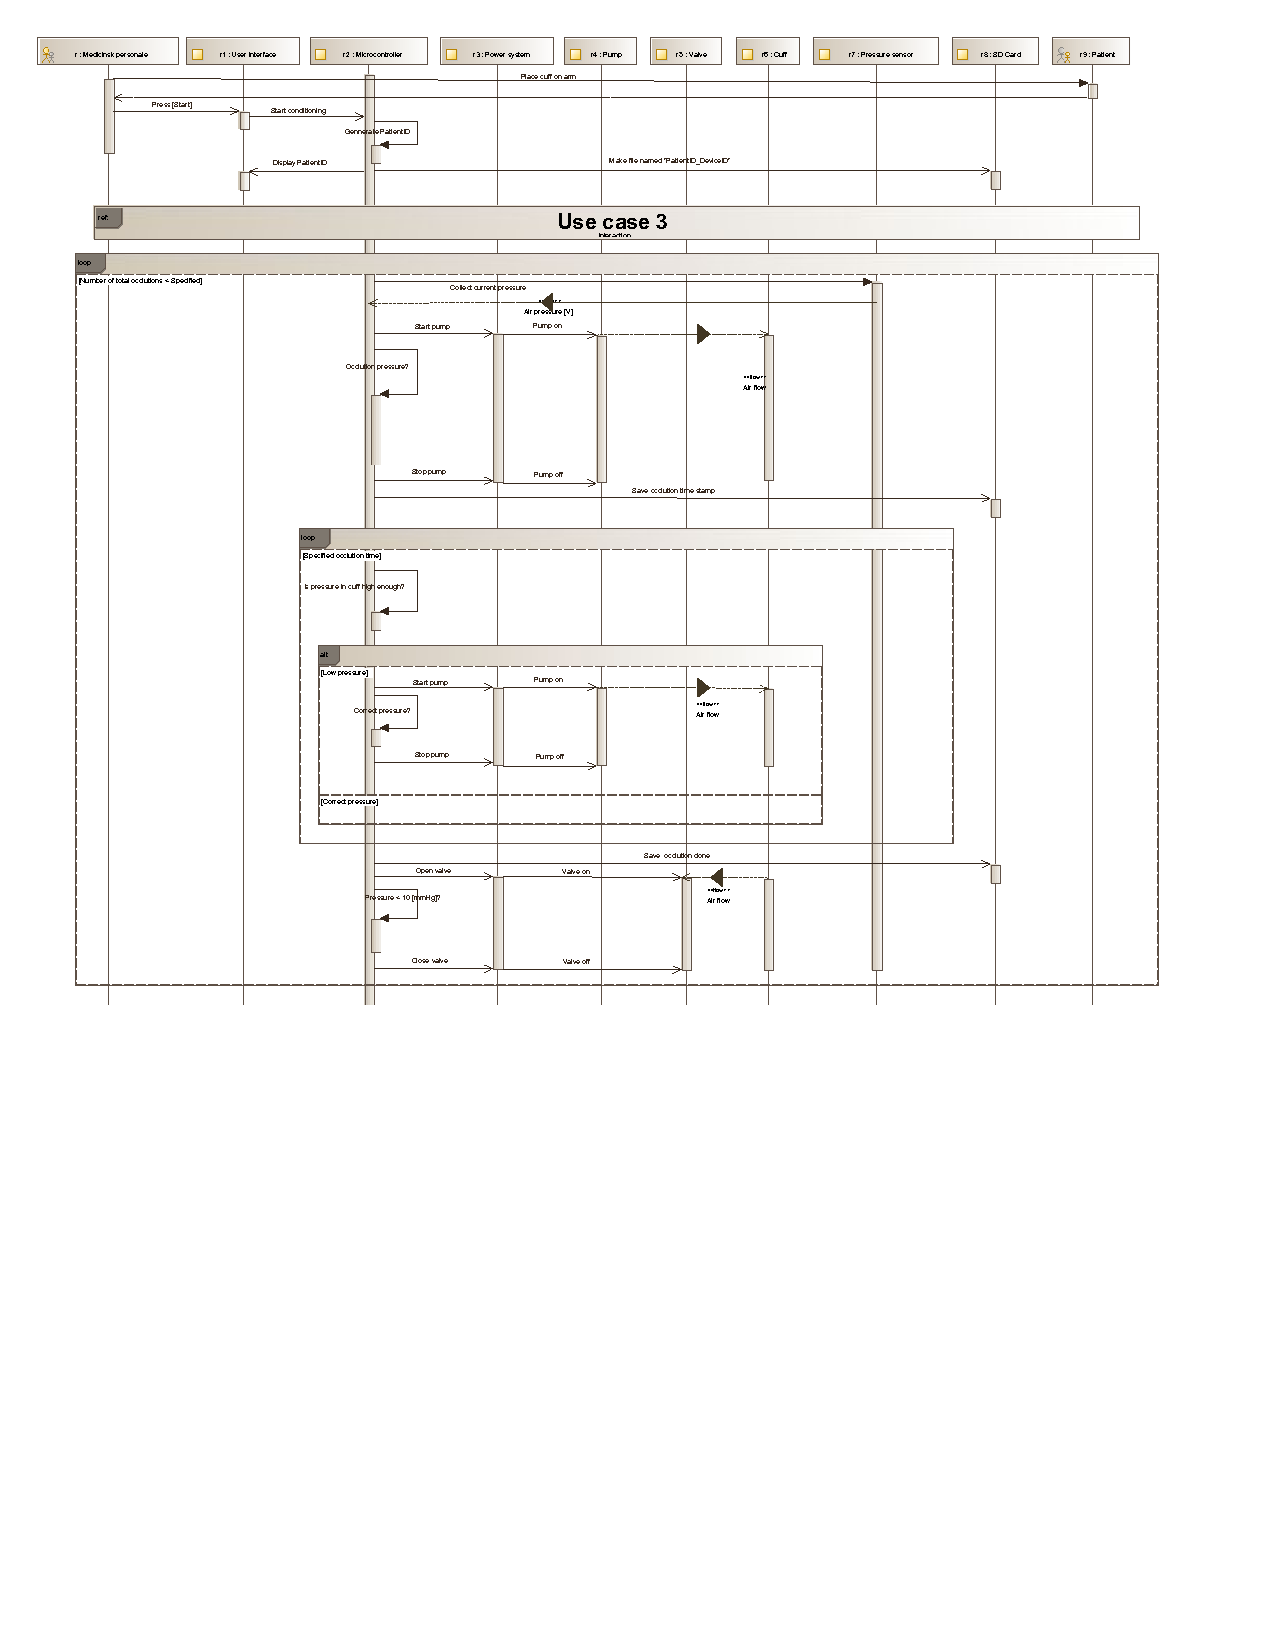
\includegraphics[width=\textwidth]{pdfs/SD_UC1-crop.pdf}

\subsection{Initialiser blodtryksmåling - UC2}
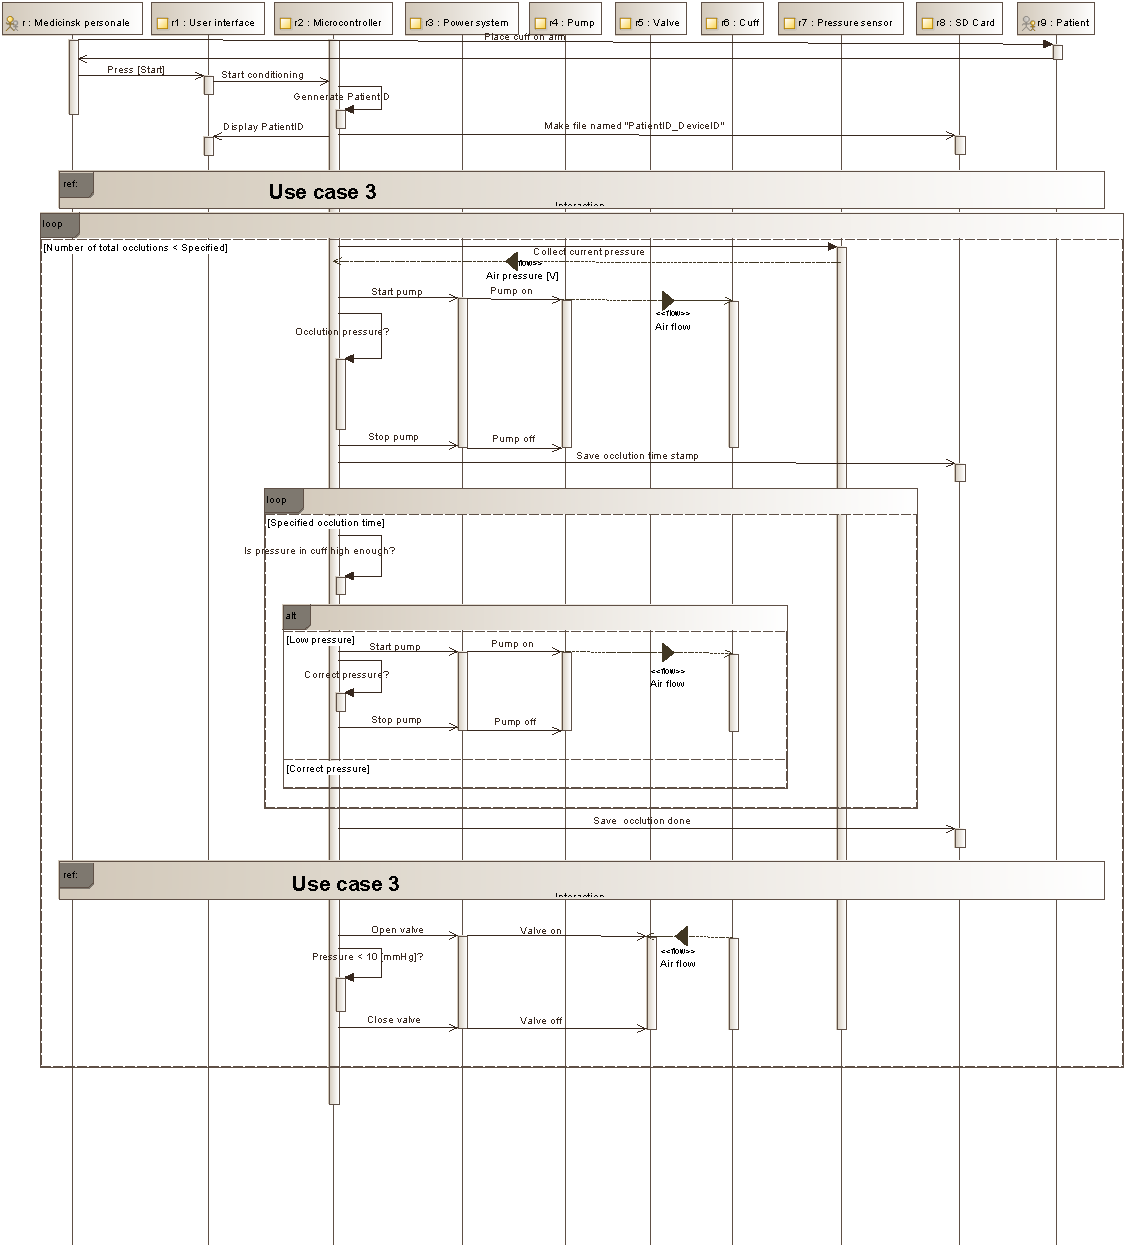
\includegraphics[width=\textwidth]{pdfs/SD_UC2-crop.pdf}

\subsection{Mål blodtryk - UC3}
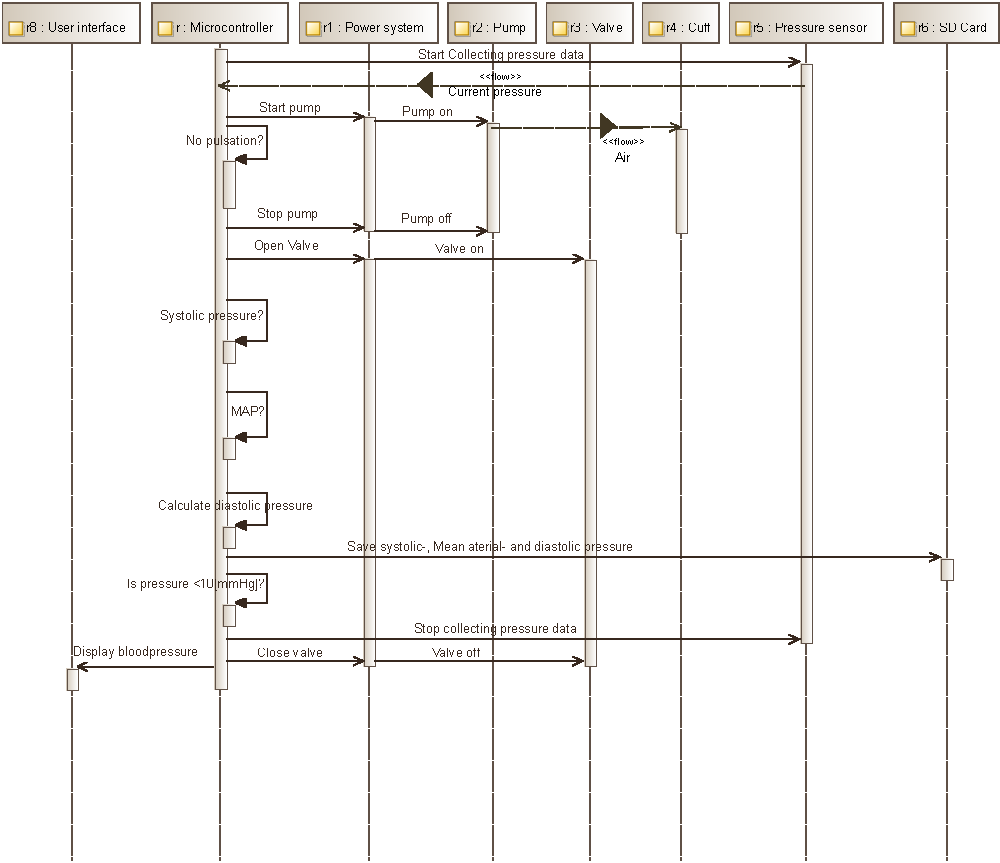
\includegraphics[width=\textwidth]{pdfs/SD_UC3-crop.pdf}

\subsection{Overfør data - UC4}
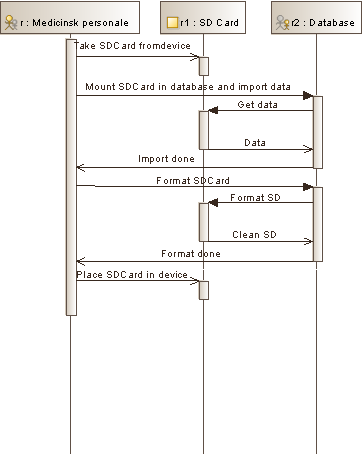
\includegraphics[width=\textwidth]{pdfs/SD_UC4-crop.pdf}

\subsection{Sikkerhedskontrol med pulsoximeter - UC5}
Mangler stadig...

\subsection{Okklusionstræning - UC6}
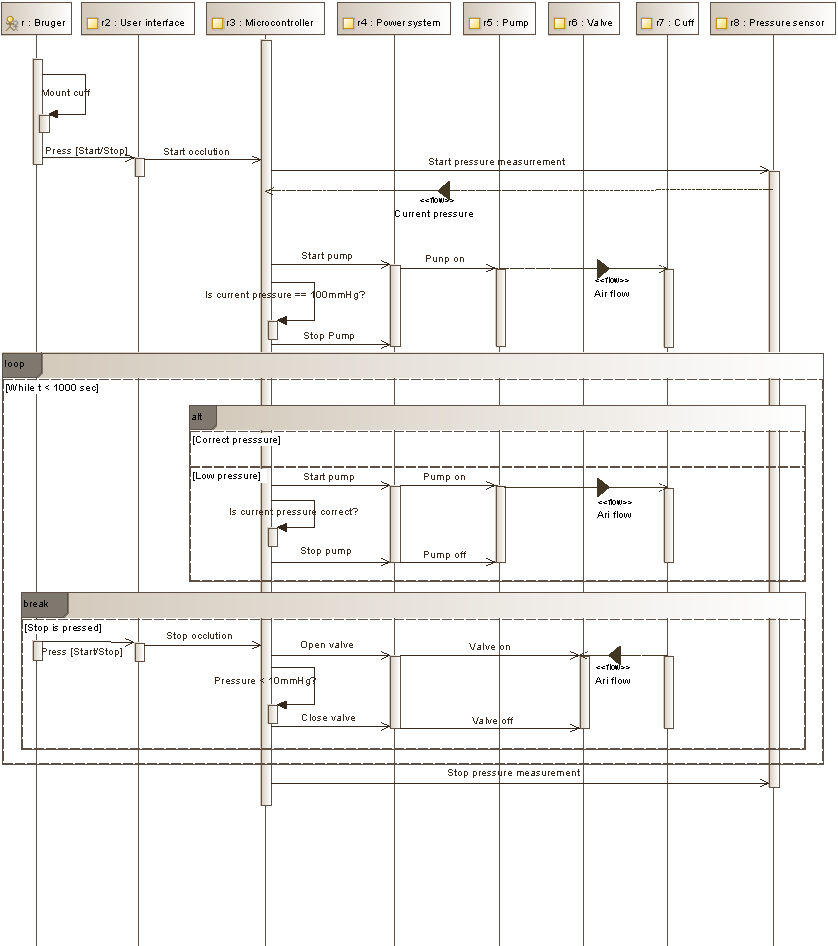
\includegraphics[width=\textwidth]{pdfs/SD_UC6-crop.pdf}

\subsection{Afbryd - UC7}
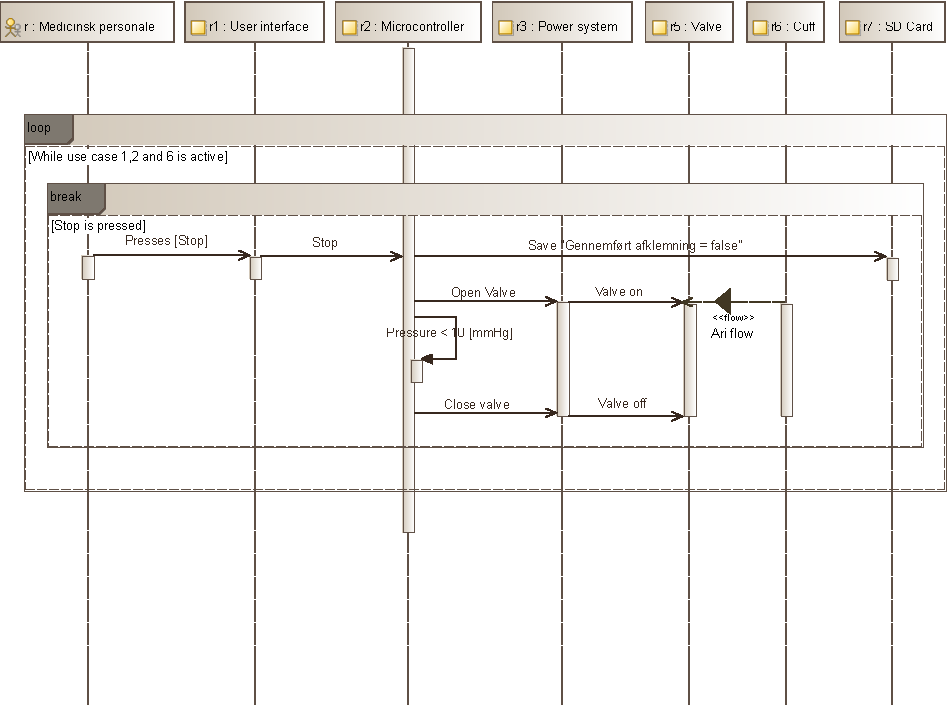
\includegraphics[width=\textwidth]{pdfs/SD_UC7-crop.pdf}

\subsection{Setup - UC8}
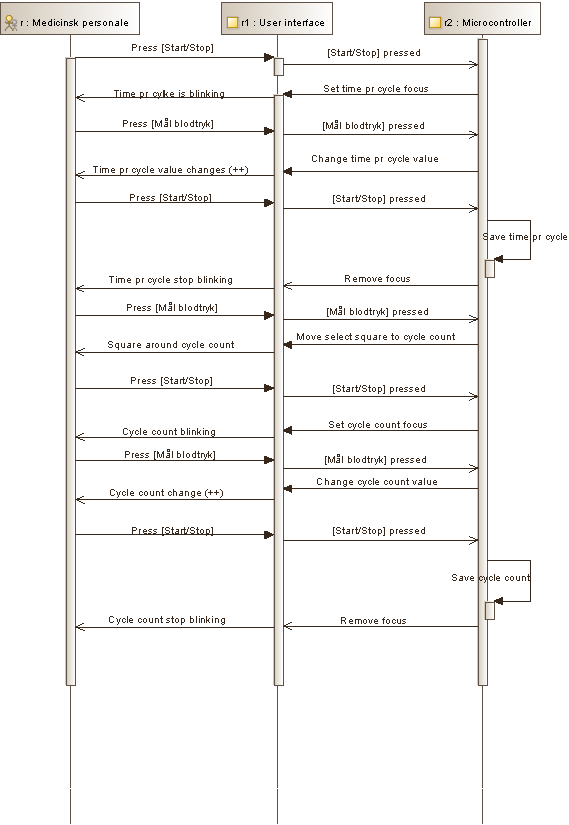
\includegraphics[width=\textwidth]{pdfs/SD_UC8-crop.pdf}
